\documentclass[10pt]{IEEEtran}

% \AtBeginDocument{%
%   \providecommand\BibTeX{{%
%       Bib\TeX}}}
% \setcopyright{acmcopyright}
% \copyrightyear{2018}
% \acmYear{2018}
% \acmDOI{XXXXXXX.XXXXXXX}

%% These commands are for a PROCEEDINGS abstract or paper.
% \acmConference[XX]{Make sure to enter the correct
%   conference title from your rights confirmation emai}{2023}{}

% \acmPrice{15.00}
% \acmISBN{978-1-4503-XXXX-X/18/06}

\usepackage{amsmath}
\usepackage{amssymb}
\usepackage{amsthm}
\usepackage{mathtools}
\usepackage{comment}
\usepackage{todonotes}
\usepackage{float}
\usepackage[algo2e,ruled,linesnumbered]{algorithm2e}

% for restatable
\usepackage{thmtools,thm-restate}
\usepackage{physics}
% %% >> for restatable links
% \usepackage{xpatch}
% \usepackage{xcolor}
% \usepackage{scalerel}

% % a flag to turn on and off
% \newif\ifmarginprooflinks
%     \marginprooflinkstrue
%     % \marginprooflinksfalse


% %% STEP 1: patch restatable so there are backward links on recall
% \makeatletter
% \xpatchcmd{\thmt@restatable}% Edit \thmt@restatable
%    {\csname #2\@xa\endcsname\ifx\@nx#1\@nx\else[{#1}]\fi}% Replace this code
%    {\ifthmt@thisistheone%
%     \csname #2\@xa\endcsname\ifx\@nx#1\@nx\else[{#1}]\fi% same as before
%     %except with also marginparbox
%    \else\fi} {}{\typeout{FIRST PATCH TO THM RESTATE FAILED}}
% \xpatchcmd{\thmt@restatable}% A second edit to \thmt@restatable
%    {\csname end#2\endcsname}
%    {\ifthmt@thisistheone\csname end#2\endcsname\else\fi}
%    {}{\typeout{FAILED SECOND THMT RESTATE PATCH}}


% \newcommand{\recall}[1]{\medskip\par\noindent{\bf \Cref{thmt@@#1}.} \begingroup\em \noindent
%    \expandafter\csname#1\endcsname* \endgroup\par\smallskip}

% %% STEP 2: make forward links to restatable.
% \setlength\marginparwidth{1.55cm}
% \let\oldmarginpar\marginpar
% \renewcommand{\marginpar}[1]{%
%     \leavevmode%
%     \oldmarginpar{#1}%
%     \ignorespacesafterend\ignorespaces}
% \newsavebox\marginprooflinkbox
% \newenvironment{linked}[3][]{%
%     \def\linkedproof{#3}%
%     \def\linkedtype{#2}%
%     \ifmarginprooflinks%
%     \sbox\marginprooflinkbox{%
%         \centering%
%         \hyperref[proof:\linkedproof]{%
%         \color{blue!30!white}%
%         \scaleleftright{$\Big[$}{\,\mbox{\footnotesize\centering\tt\begin{tabular}{@{}c@{}}
%             link to\\[-0.15em]
%             proof
%         \end{tabular}}\,}{$\Big]$}}~}
%     \fi
%         \restatable[#1]{#2}{#2:#3}\label{#2:#3}%
%     \reversemarginpar	\ifmarginprooflinks\marginpar{\vspace{-1ex}\usebox\marginprooflinkbox}\fi
%     }%
%     {\sbox\marginprooflinkbox{}\endrestatable}
% \newcounter{proofcntr}
% \newenvironment{lproof}{\begin{proof}\refstepcounter{proofcntr}}{\end{proof}}

\newcommand{\vect}[1]{\ensuremath{\mathbf{#1}}}

%% Useful
\newcommand{\p}[1]{\left( #1 \right)}
\newcommand{\br}[1]{\left[ #1 \right]}


%\newcommand{\ev}[1]{\mathbb{E}\left[{#1}\right]}
\newcommand{\evd}[2]{\mathbb{E}_{#1}\left[{#2}\right]}

%% Algortihm notations
\newcommand{\bigO}[1]{O \left( #1 \right )}

%% Calibration
\newcommand{\I}[1]{\mathbb{I}\left[#1\right]}       % Indicator
\newcommand{\calerr}{\mathrm{calerr}}   % Calibration error

\newcommand{\A}{\mathcal{A}}    % Algorithm
\newcommand{\Ber}{\mathrm{Ber}}
\newcommand{\Ecover}{\event^{\textrm{cover}}}   % Event that covered epochs exist
\newcommand{\Enegl}{\event^{\textrm{negl}}}     % Event that negligible epochs exist
\newcommand{\Epoch}{\mathsf{Epoch}}
\newcommand{\eps}{\epsilon}     % epsilon
\newcommand{\Etruth}{\event^{\textrm{truth}}}   % Event that all epochs are truthful
\newcommand{\event}{\mathcal{E}}    % Events
\newcommand{\Ex}[2]{\operatorname*{\mathbb{E}}_{#1}\left[#2\right]}  % Expectation
\newcommand{\Int}{\mathcal{I}}      % Interval
\newcommand{\poly}{\operatorname*{poly}}    % Polynomial
\newcommand{\pr}[1]{\Pr\left[#1\right]}     % Probability
%\newcommand{\red}[1]{{\color{red} #1}}

\newcommand{\red}[1]{\textcolor{red}{#1}}
\newcommand{\blue}[1]{\textcolor{blue}{#1}}

\newcommand{\SPinner}{\mathsf{SP}^{\textrm{inner}}}
\newcommand{\SPouter}{\mathsf{SP}^{\textrm{outer}}}
\newcommand{\Tact}{T^{\mathrm{actual}}}     % Actual stopping time
\newcommand{\prodspace}{\mathcal{X}\times A \times \mathcal{Y}}


%% Fair ERM Notation
\newcommand{\error}[1]{ \left| \mathbb{E}_{(x,y) \sim \mathcal{D}} \ [\one (#1(x) \neq y)] - \ \mathbb{E}_{(x,y) \sim \mathcal{D}} \ [\one (h^*(x) \neq y)] \right|}
\newcommand{\htilde}{\tilde{h}}
\newcommand{\hhat}{\hat{h}}
\newcommand{\hstar}{h^*}
\newcommand{\hclass}{\mathcal{H}}
\newcommand{\posrate}[1]{ P_{(x,y) \sim \DA} [#1 (x)=1]}

\newcommand{\DAC}{\widetilde{\mathcal{D}}_A}
\newcommand{\DBC}{\widetilde{\mathcal{D}}_B}
\newcommand{\RA}{P_{(x,y) \sim \dist } [x \in A]}
\newcommand{\RB}{P_{(x,y) \sim \dist} [x \in B]}
\newcommand{\normalF}{F}
\newcommand{\corruptF}{\widetilde{F}}




\title{Formal description of ML models for unambiguous implementation}           
\author{
  \IEEEauthorblockN{Adrien Gauffriau}
  \IEEEauthorblockA{\textit{Airbus, France}}
  \and
   \IEEEauthorblockN{Iryna De Albuquerque Silva}
  \IEEEauthorblockA{\textit{ONERA, France}}
  \and
  \IEEEauthorblockN{Claire Pagetti}
  \IEEEauthorblockA{\textit{ONERA, France}}
}



\begin{document}
\maketitle

% \begin{abstract}

The Fast Reciprocal Square Root Algorithm is a well-established approximation technique consisting of two stages: first, a coarse approximation is obtained by manipulating the bit pattern of the floating point argument using integer instructions, and second, the coarse result is refined through one or more steps, traditionally using Newtonian iteration but alternatively using improved expressions with carefully chosen numerical constants found by other authors. The algorithm was widely used before microprocessors carried built-in hardware support for computing reciprocal square roots. At the time of writing, however, there is in general no hardware acceleration for computing other fixed fractional powers. This paper generalises the algorithm to cater to all rational powers, and to support any polynomial degree(s) in the refinement step(s), and under the assumption of unlimited floating point precision provides a procedure which automatically constructs provably optimal constants in all of these cases. It is also shown that, under certain assumptions, the use of monic refinement polynomials yields results which are much better placed with respect to the cost/accuracy tradeoff than those obtained using general polynomials. Further extensions are also analysed, and several new best approximations are given.

\end{abstract}



\section{Introduction}
Current quantum hardware is unable to carry out universal quantum computations due to the buildup of errors that occur during the computation. 
The magnitude of the individual error is currently above the value that the Threshold Theorem requires in order to kick-start quantum error correction and fault-tolerant quantum computation~\cite[Section 10.6]{nielsen_chuang_2010}. 
Although the experimentally achieved fidelity rates are promising and the error bounds are inching closer to the required threshold, we will have to work for the foreseeable future with quantum hardware with errors that build-up during the computation.  This implies that we can only do a limited number of steps before the output of the computation has become completely uncorrelated with the intended one.

For fault-tolerant quantum computing, we repeat four steps: 
1) We apply a number of single and two-qubit quantum gates, in parallel whenever possible; 
2) We perform a syndrome measurement on a subset of the qubits; 
3) We perform fast classical computations to determine which errors have occurred and how to correct them; 
and, 4) We apply correction terms based on the classical computations.
We then repeat these four steps with a next sequence of gates. 
These four steps are essential to fault-tolerant quantum computing. 


The starting point of this work is to use the four steps outlined above, not to carry out error correction and fault-tolerant computation, but to enhance short, constant-depth, {\em uncorrected} quantum circuits that perform single qubit gates and {\em nearest-neighbor} two qubit gates. 
Since in the long run we will have to implement error-correction and fault-tolerant computation anyhow, and this is done by such a four-step process, why not make other use of this architecture? Moreover, on some of the quantum hardware platforms, these operations are already in place.
Embracing this idea we naturally arrive at the question: what is the computational power of \textit{low-depth} quantum-classical circuits organized as in the four steps outlined above? 
We thus investigate circuits that execute a small, ideally constant, number of stages, where at each stage we may apply, in parallel, single qubit gates and {\em nearest-neighbor} two qubit gates, followed by measurements, followed by low-depth classical computations of which the outcome can control quantum gates in later stages. 
It is not clear, at first, whether such circuits, especially with constant depth, can do anything remotely useful. 
But we will see that this is indeed the case: many quantum computations can be done by such circuits in constant depth. 
By parallelizing quantum computations in this way, we improve the overall computational capabilities of these circuits, as we do not incur errors on qubits that are idle, simply because qubits are not idle for a very long time. 
Furthermore, reducing the depth of quantum circuits, at the cost of increasing width, allows the circuit to be run faster even if errors occur.

The first usage of such a four-step layout, not to do error correction, but to perform computations, can be found in the paradigm of measurement-based quantum computing~\cite{gottesman1999demonstrating,raussendorf2001one,jozsa2006introduction,clark2007generalised}: 
A universal form of quantum computing where a quantum state is prepared and operations are performed by measuring qubits in different bases, depending on previous measurements and intermediate measurements.

\citeauthor{PhamSvore2013} were the first to formalize the four-step protocol for performing computations~\cite{PhamSvore2013}. They included specific hardware topologies by considering two-dimensional graphs for imposing constraints on qubit interactions. In their model, they develop circuits for particularly useful multi-qubit gates, including specifying costs in the width, number of qubits, depth, number of concurrent time steps, size, and total number of non-Identity operations.
As a result, they find an algorithm that factors integers in polylogarithmic depth.
\citeauthor{Browne:2011} showed that the main tool in the work by \citeauthor{PhamSvore2013}, the fan-out gate, can also be replaced by additional log-depth classical computations in the measurement-based quantum computing setting~\cite{Browne:2011}.

More recently, \citeauthor{Cirac:2021} introduced a scheme to implement unitary operations involving quantum circuits combined with Local Operations and Classical Communication ($\mathsf{LOCC}$) channels: $\mathsf{LOCC}$-assisted quantum circuits~\cite{Cirac:2021}. Similarly to the four-step scheme we just described, they allow for a short depth circuit to be run on the qubits, followed by one round of $\mathsf{LOCC}$, in which ancilla qubits are measured and local unitaries are applied based on the measurement outcomes. They show that in this model any 1D transitionally invariant matrix-product state (MPS) with fixed bond dimension is in the same phase of matter as the trivial state. Similar ideas can be found in~\cite{TVV_NonAbelianTopologicalOrder_2022, tantivasadakarn2021long}.

In this work, we introduce a new model, called \textit{Local Alternating Quantum-Classical Computations} ($\LAQCC$). In this model we alternate between running quantum circuits (constrained by locality), ending in the measurement of a subset of qubits, and fast classical computations based on the measurement results. The outcome of the classical computations are then used to control future quantum circuits. We allow for flexibility in this model, by giving different constraints to the power of both the quantum circuits and the classical circuits as well as the number of alternations between them. 
Most attention will be given to $\LAQCC$ containing quantum circuits of constant depth, classical circuits of logarithmic depth and at most a constant number of alternations between them. 
Any circuit constructed in this model is considered to be of constant depth. 
We restrict ourselves to logarithmic depth classical computations, as this is the first natural and non-trivial extension beyond constant-depth classical computations. 
Constant-depth classical computations do however also have an equivalent constant-depth quantum implementation.

The definition of $\LAQCC$ sharpens the original definition of \citeauthor{PhamSvore2013} by adding constraints to the intermediate classical computations. This allows us to bound the power of $\LAQCC$ from above. 

The main result of \citeauthor{Cirac:2021}, that 1D translational invariant MPS with fixed bond dimension can be prepared by $\mathsf{LOCC}$-assisted circuits, relies on local symmetries of the MPS. These symmetries allow them to prepare local states (on a constant number of qubits) and glue them together by doing one round of the appropriate entangling measurement and corrections, after which they run a round of local unitaries to get the desired result. This general scheme for preparing states that exhibit an MPS description with the appropriate local symmetries requires only geometrically local unitaries and one round of measurement and corrections an therefore is accessible in $\LAQCC$. Studying different local symmetries, known as Symmetry Protected Topological (SPT) phases of matter, to find measurement-based constant depth circuits for states is a broad ongoing field of research~\cite{TVV_NonAbelianTopologicalOrder_2022, tantivasadakarn2021long, smith2023deterministic}. 
All these schemes have a $\LAQCC$ implementation.

%$\LAQCC$-circuits also exist for general schemes of preparing local states, based on the local tensors, and gluing them together using one round of entangled measurement and corrections, based on the local symmetry. 
%The main result of \citeauthor{Cirac:2021}, that 1D translational invariant MPS with fixed bond dimension can be prepared by $\mathsf{LOCC}$-assisted circuits, relies heavily on local symmetries of the MPS and as a result also has an equivalent $\LAQCC$ implementation. 
%The corrections applied after the measurement round are local unitaries depending on the local symmetries of the MPS. 

 

%This general scheme of preparing local states, based on the local tensors, and gluing it together by doing one round of entangled measurement and corrections, based on the local symmetry, is accessible in $\LAQCC$.
Note however that \citeauthor{Cirac:2021} also suggest a circuit for the $W$-state.
This circuit uses sequentially and dependent measurement-based corrections of the ancilla qubits. 
These dependent measurements translate to sequential alternations between the quantum and classical circuits and therefore increase the total depth to linear depth, exceeding the constant-depth constraints imposed by $\LAQCC$-circuits. 

We study the power of the $\LAQCC$ model with respect to state preparation, showing that even with only constant quantum-depth and logarithmic classical depth it remains possible to prepare states with long-range entanglement.
Another surprising result is that it is unlikely that $\LAQCC$ circuits are classically simulatable. We show that any instantaneous quantum polynomial-time (IQP) circuit~\cite{Bremner2010,Shepherd2009} has an $\LAQCC$ implementation.
Classical simulation of IQP circuits implies the collapse of the polynomial hierarchy to the third level, which is not believed to be true~\cite{Bremner2017}. Therefore, we expect that $\LAQCC$ circuits are unlikely to be classically simulatable. We bound the power of $\LAQCC$ by showing that it is contained in $\QNC^1$, the class of polynomial-size, log-depth circuits.

Next, we also study the power that intermediate classical calculations can add to quantum computations, by considering a new model that alternates between polynomially many polynomial-depth quantum circuits and unbounded classical computations
We study this model by doing a complexity theoretical analysis, where we draw inspiration from the notions of complexity given by \citeauthor{RosenthalYuen:2022}, \citeauthor{MetgerYuen:2023}, and \citeauthor{Aaronson:2004}.
All three complexity notions are based on the notion of state preparation, instead of more traditional definition of complexity such as the decidability of a computational problem. 
The first two consider classes based on sequences of quantum states preparable by a polynomial-sized quantum circuit, where the circuits are uniformly generated by a computational class, for instance, the class $\mathsf{PSPACE}$, which results in the complexity class $\mathsf{StatePSPACE}$~\cite{RosenthalYuen:2022,MetgerYuen:2023}.
The third notion considers a relative complexity, where the complexity is measured between two given states, and is measured by the number of gates, from a given gate-set, required to transform one state in another state~\cite{Aaronson:2004}. 
For our definition of state preparation complexity, we drop the uniformity constraint from~\cite{RosenthalYuen:2022,MetgerYuen:2023} and define a class as $\mathsf{StateX}$, which refers to states preparable by circuits of type $\mathsf{X}$. 
As an example, if $\mathsf{X} = \QNC^0$, this results in the class $\mathsf{StateQNC^0}$, which is the set of states preparable from the $\ket{0}^n$ state by poly-size constant-depth circuits. 
This notion is similar to the relative complexity from~\cite{Aaronson:2004}, where one state is the  $\ket{0}^n$ state and instead of counting the number of gates we consider the set of states preparable by a fixed number of gates. Using this notion of complexity we show that any state preparable by an $\LAQCC^*$ circuit is also preparable by a $\mathsf{PostQPoly}$ circuit, the class of circuits of polynomial depth with an additional post-selection gate. 

All Clifford circuits have a constant-depth $\LAQCC$ implementation, implying that any stabilizer state can be implemented by a constant-depth $\LAQCC$ circuit, see Section~\ref{sec:clifford_circuits} for a proof of this statement. 
Efficient circuits for stabilizer states have been known already through measurement-based quantum computing. Therefore this paper focuses on the preparation of non-stabilizer states, and as a surprising result we find novel constant-depth protocols for four very natural classes of non-stabilizer states.
Despite the extensive research into these four classes of non-stabilizer states and the many applications of them, no efficient constant- or low-depth state preparation protocols are known yet. We specifically consider these four classes as they are all often used as initial states in other algorithms.

The first state is a uniform superposition over an arbitrary number of states. 
This state finds applications in many quantum algorithms, as they often start with a uniform superposition over multiple states. 
This superposition is often achieved by applying Hadamard gates to every qubit due to its simplicity to prepare. 
Yet, the analysis of many algorithms, such as Shor's algorithm~\cite{Shor:1997}, would benefit from a different initial superposition. 
The circuit to prepare the uniform superposition over an arbitrary number of states uses an exact version of Grover search as a subroutine, that turns a probabilistic circuit, with a known constant probability of success, into a deterministic circuit. 
We use the circuit for preparing a uniform superposition over an arbitrary number of states as a subroutine in the next two quantum state preparation protocols. 

The second state is the $W$-state, the uniform superposition over all computational basis states of Hamming-weight~$1$, a natural long-ranged entangled state that displays a fundamentally nonequivalent type of entanglement from the Greenberger–Horne–Zeilinger state~\cite{WState:2000}, for which $\LAQCC$-type constant-depth circuits were previously known~\cite{PhamSvore2013, Cirac:2021}. 
The $W$-state is often used as benchmark for new quantum hardware~\cite{Haffner2005,Neeley2010,GarciaPerez:2021}. 
A novel way to prepare the $W$-state therefore gives a new way to benchmark different quantum devices with each other. 
A circuit for preparing the $W$-state was given in~\cite{Cirac:2021}, but this implementation requires sequentially alternating measurements followed by local unitaries, which in the $\LAQCC$ model is not considered to be of constant depth. 
We improve this protocol by giving an $\LAQCC$ implementation of the $W$-state, based on a compress-uncompress method that links the one-hot and binary encoding of integers.

The third state considered is the Dicke state, a generalization of the $W$-state, a superposition over all computational basis states with Hamming-weight $k$~\cite{Dicke:1954}. 
Dicke states have relevance in various practical settings.
For instance, for quantum game theory~\cite{zdemir2007}, quantum storage~\cite{Bacon_Compress:2006,Plesch:2010}, quantum error correction~\cite{ouyang2014permutation}, quantum metrology~\cite{toth2012multipartite}, and quantum networking~\cite{prevedel2009experimental}. 
Dicke states have been used as a starting state for variational optimization algorithms, most notably Quantum Alternating Operator Ansatz (QAOA)~\cite{Hadfield2019}, to find solutions to problems such as Maximum k-vertex Cover~\cite{Brandhofer2022,cook2020quantum}.
The ground states of physical Hamiltonians describing one-dimensional chains tend to show a resemblance to Dicke states such as states resulting from the Bethe ansatz, making them an ideal starting state when investigating the ground state behavior of these Hamiltonians~\cite{TDL_BetheAnsatzDerivation:2010,B_ExcitedStateQuantumPhaseTransitions:2013,DickeTransitions:2021}. 
For instance, the algorithm by \citeauthor{van2021preparing}, who give an algorithm to prepare the Bethe ansatz eigenstates of the spin-1/2 XXZ spin chain, starts by first preparing a Dicke state~\cite{van2021preparing}. 
A Dicke-state preparation protocol based on the compress-uncompress methodology used in the $W$-state furthermore finds applications in entanglement distillation, where the entanglement of a large state is concentrated on only a few qubits. 
Efficient deterministic circuits for preparing Dicke states have been proposed by \citeauthor{bartschi2019deterministic}~\cite{bartschi2019deterministic, bartschi2022deterministic_short_depth}. 
They provide a quantum circuit of depth $\mathO(k \log(\frac{n}{k}))$, allowing arbitrary connectivity, to prepare a Dicke state, which they conjecture to be optimal when $k$ is constant. 
In this work, we provide a constant-depth $\LAQCC$ circuit below their conjectured bound already for constant $k$. 
However, this does not directly disprove their conjecture, as we allow for intermediate measurements and classical computations. 
More significantly, we even construct constant-depth $\LAQCC$ circuits for $k = \mathO(\sqrt{n})$ greatly improving their bound.
This construction extends the compress-uncompress method for the $W$-state combined with additional subroutines. 

We continue with a log-depth state preparation protocol for the Dicke-state for arbitrary $k$. 
This protocol implements an efficient transformation between the factoradic number representation and the combinatorial number representation of a positive integer. 
The combinatorial number representation relates directly to the Dicke state. 
The provided efficient transformation between number representation systems might be of independent interest. 

We conclude by modifying our protocol for preparing a Dicke-state to a protocol that prepares quantum many-body scar states in constant-depth. 
These states have low entanglement and longer coherence times than states with similar energy density.
These characteristics make many-body scar states interesting to analyze and relevant within physics.
Many-body scar states appear for instance in the AKLT model~\cite{AKLT:1987,MRBAR:2018,MRB:2018} and different spin models~\cite{SI:2019,MOBFR:2020}.
Known methods for preparing these states have polynomial-depth~\cite{Gustafson:2023}, whereas our circuit has constant depth. 

% We conclude by studying the power that intermediate classical calculations can add to quantum computations. 
% In this study, we define a new model that relaxes constant-depth quantum circuits to polynomial depth quantum circuits, log-depth classical calculations to unbounded classical computations and a constant number of alternations to a polynomial number of alternations. 
% We call this model $\LAQCC^*$. 
% We study this model by doing a complexity theoretical analysis, where we draw inspiration from the notions of complexity given by \citeauthor{RosenthalYuen:2022}, \citeauthor{MetgerYuen:2023}, and \citeauthor{Aaronson:2004}.
% All three complexity notions are based on the notion of state preparation, instead of more traditional definition of complexity such as the decidability of a computational problem. 
% The first two consider classes based on sequences of quantum states preparable by a polynomial-sized quantum circuit, where the circuits are uniformly generated by a computational class, for instance, the class $\mathsf{PSPACE}$, which results in the complexity class $\mathsf{StatePSPACE}$~\cite{RosenthalYuen:2022,MetgerYuen:2023}.
% The third notion considers a relative complexity, where the complexity is measured between two given states, and is measured by the number of gates, from a given gate-set, required to transform one state in another state~\cite{Aaronson:2004}. 
% For our definition of state preparation complexity, we drop the uniformity constraint from~\cite{RosenthalYuen:2022,MetgerYuen:2023} and define a class as $\mathsf{StateX}$, which refers to states preparable by circuits of type $\mathsf{X}$. 
% As an example, if $\mathsf{X} = \QNC^0$, this results in the class $\mathsf{StateQNC^0}$, which is the set of states preparable from the $\ket{0}^n$ state by poly-size constant-depth circuits. 
% This notion is similar to the relative complexity from~\cite{Aaronson:2004}, where one state is the  $\ket{0}^n$ state and instead of counting the number of gates we consider the set of states preparable by a fixed number of gates. Using this notion of complexity we show that any state preparable by an $\LAQCC^*$ circuit is also preparable by a $\mathsf{PostQPoly}$ circuit, the class of circuits of polynomial depth with an additional post-selection gate. 

\paragraph{Summary of results}
\begin{itemize}
    \item We give a new definition of a computational model that captures the power of the four step process: applying a constant number of layers of one- and two-qubit gates; performing a syndrome measurement; perform a fast classical computation determining corrections; apply corrections. We call this model \emph{Local Alternating Quantum Classical Computations}, or $\LAQCC$ for short. In this model we bound the allowed quantum operations, intermediate classical calculations, and number of rounds separately. In Section~\ref{sec:LAQCC_model} we define this model and give a list of operations based on results from literature contained in this computational model. In some of these operations we explicitly use that we allow for multiple, but at most constant, rounds  of corrections.
    \item  We show show that there exist $\LAQCC$ circuits that can not be weakly simulated in Section~\ref{sec:IQP_in_LAQCC}. We further show that for every $\LAQCC$ circuit there exists a $\QNC^1$ circuit simulating it perfectly, in Section~\ref{sec:LAQCC_in_QNC1}.
    \item We introduce a new type computational complexity for preparing states and show that the extension of $\LAQCC$ where we allow a polynomial number of rounds and unbounded classical computation, is contained in $\mathsf{PostQPoly}$, the class of polynomial circuits with post-selection, in Section~\ref{sec:Complexity results}.
    \item We show a protocol to prepare the uniform superposition state of size $q$ in $\LAQCC$ using $\mathO(\ceil{\log_2(q)}^2)$ qubits in Section~\ref{sec:superposition_modulo_q}. 
    \item We show a protocol to prepare the $W_n$ state in $\LAQCC$ using $\mathO(n\log(n))$ qubits in Section~\ref{sec:W_state_in_LAQCC}.
    \item We show two ways of preparing the Dicke-$(n,k)$ state. The first method is in $\LAQCC$, works up to $k = \mathO(\sqrt{n})$, uses $\mathO(n^2\log(n))$ qubits, and is found in Section~\ref{sec:dicke:small_k}. The second method is in $\LAQCC\text{-}\mathsf{LOG}$ (an extension of $\LAQCC$ allowing for logarithmic number of alterations instead of constant), works for any $k$, uses $\mathO(\text{poly}(n))$ qubits, and is found in Section~\ref{sec:Dicke_in_LAQCC_LOG}. 
    \item We extend on our $\LAQCC$ method of generating Dicke-$(n,k)$ states for $k = \mathO(\sqrt{n})$ and show a protocol to generate many-body scar states for a particular Hamiltonian in $\LAQCC$ (Section~\ref{sec:many_body_scar}). 
\end{itemize}
Summarized in a table, we provide the following state generation protocols:
\begin{table}[htb]
\centering
\begin{tabular}{l|l|l|l}
\textbf{State description} & \textbf{Width} & \textbf{Depth} & \textbf{Implementation}\\
\hline 
Uniform superposition mod $q$: $\frac{1}{\sqrt{q}} \sum_{i = 0}^{q-1}\ket{i}$ & $\mathO(\ceil{\log^2 q})$ & $\mathO(1)$ & Section~\ref{sec:superposition_modulo_q}\\

$W$-state: $\frac{1}{\sqrt{n}}\sum_{i = 0}^{n-1}\ket{e_i}$ & $\mathO(n \log n)$ & $\mathO(1)$ & Section~\ref{sec:W_state_in_LAQCC}\\

Dicke-$(n,k)$, $k = \mathO(\sqrt{n})$: $\binom{n}{k}^{-1/2}\sum_{x \in \{0,1\}^n: |x| = k} \ket{x}$ &  $\mathO(n^2\log n)$ & $\mathO(1)$ 
&Section~\ref{sec:dicke:small_k}\\

Dicke-$(n,k)$: $\binom{n}{k}^{-1/2}\sum_{x \in \{0,1\}^n: |x| = k} \ket{x}$ & $\mathO(\text{poly}(n))$ & $\mathO(\log n)$ &Section~\ref{sec:Dicke_in_LAQCC_LOG}\\

QMBS: $\ket{S_k} = \frac{1}{k! \sqrt{\mathcal N(n,k)}}(Q^\dagger)^k \ket{\Omega}$ &  $\mathO(n^2\log n)$ & $\mathO(1)$  &  Section~\ref{sec:many_body_scar}
\end{tabular}
\caption{Summary of state preparation protocols given in this paper.}
\label{tab:sate_prep}
\end{table}
In the entry for the quantum many-body scar state $Q$ denotes the raising operator and $\mathcal N(n,k)=\binom{n-k-1}{k}$. 
Section~\ref{sec:many_body_scar} will provide more details on the variables and the implementation. 

\paragraph{Organization of the paper}
\noindent We first introduce relevant preliminaries in Section~\ref{sec:preliminaries}. 
In Section~\ref{sec:LAQCC_model} we formally define the class of Local Alternating Quantum-Classical Computations ($\LAQCC$). We also show that any Clifford circuit can be implemented in constant depth $\LAQCC$ (a result based on a result from measurement-based quantum computing~\cite{jozsa2006introduction}). 
This result allows us to give many useful multi-qubit gates and routines in Section~\ref{sec:gates_created_in_LAQCC}. 
Beyond that we show that constant depth $\LAQCC$ circuits are contained in $\QNC^1$ and that any $\mathsf{IQP}$ circuit has an $\LAQCC$ implementation.
We conclude this section with an analysis of a more powerful instantiation of $\LAQCC$ and show an inclusion with respect to the class $\mathsf{PostQPoly}$, which is the class of circuits of polynomial depth with one additional post-selection gate. 
In Section~\ref{sec:state_prep_in_LAQCC} we give $\LAQCC$ circuit implementations for preparing the uniform superposition over an arbitrary number of states, the $W$-state and the Dicke state up to $k = \mathO(\sqrt{n})$. We furthermore give a log-depth circuit implementation for preparing the Dicke state for any $k$. We conclude by showing a $\LAQCC$ circuit for generating many body scar states of a particular type of Hamiltonian.


\section{Format of description -- \nnef}
\label{sec-nnef}
% Peut être ne pas tout définir, mais essayer de faire un truc un peu plus minimal.
% Rajouter le fait que le noeud s'active quand on recoit un nouvel input.
\khronos standardization group\footnote{\url{https://www.khronos.org/}} has defined the \nnef (Neural Network Exchange format)
format with a specification that provides a syntax and a semantic.
%After outlining the definition of deep neural network, we will present \nnef.
We focus on the \nnef syntax and semantics elements needed for our purpose. The reader can refer
to \cite{nnefformat} for a complete description of \nnef.
%We end the section by defining the execution model semantics
%with a translation into \petri net.

\subsection{Brief Reminder on Neural Network}

% From Iryna proposal, MAJ 12/02

The field of artificial intelligence has gained much research attention in the past years.
The power of AI resides in the capacity of solving highly complex problems \cite{Goodfellow-et-al-2016}. 
%In contrast, tasks that rely on intuitive reasoning, which can easily achieved by humans but that are hard to describe formally, represent a real challenge.
%Within artificial intelligence,
Machine learning domain describes the study and development of statistical algorithms that are able to efficiently generalize on unknown input data after the extraction of patterns from a similar, and representative, data set.
%Examples of tasks where ML succeeds are detecting a runway in an image for aircraft landing \cite{aerospace9110634}, supporting predictive maintenance \cite{Carvalho2019-pi}, helping air traffic control \cite{Yousefzadeh2021} or yet understanding spoken commands \cite{Nassif2019}. 
%The capability of generalizing -- or \emph{inferring} -- well derives from a \emph{learning} -- or \emph{training} -- process.
%, which is an optimization problem \cite{Mitchell1997-ux}.
Neural networks are a class of ML algorithms. A neural network implements a mathematical function \Fn that aims at approximating a continuous real-valued function \cite{Hornik1989, Schafer2006}. 
%The term network comes from the fact that
\Fn is  composed of  different mathematical functions called \emph{layers}.
%Each function composing \Fn is associated to a \emph{layer}.
 %The number of layers in a neural network defines its \emph{depth}.
%Deep neural networks are then neural networks with multiple hidden layers. 
%The number of units acting in parallel in each layer define the neural network \emph{topology}.
%The objective is that some parameters of function \Fn be recursively updated resulting in an accurate function approximation. This optimization process is called \emph{training}. 


There are two types of deep neural networks: feed-forward neural networks and recurrent neural networks. 
Recurrent neural networks (RNN) feature layers that take as input some of their output (or the output of a successor layer), thus creating cycles. In feed-forward variants it is not true. We are not addressing RNN in this paper.
A common representation of a feed-forward deep neural network (FDNN) is in the form of a \emph{directed acyclic graph} (DAG) defining how its layers are connected together.
%Then we associate a mathematical function \Fn to this directed graph, describing the mathematical rules of the neural network. 

\begin{definition}[Feed-forward Deep Neural Network] \label{def:dnn}
  \it
  A \emph{feed-forward deep neural network} $\mathcal{N}=(V,E)$ is a directed acyclic graph, wherein:
  \begin{itemize}
  \item $V$ is the finite set of vertices of the graph, which represent its layers $l \in V$;
  \item $E\subseteq V\times V$ is the set of edges of the graph, representing the data flow within the neural network.
  \end{itemize} 
\end{definition}

In order to construct the possible flows of data within the feed-forward deep neural network, it is necessary to define what are the predecessors and successors of a vertex, or layer. 

\begin{definition}[Predecessors / successors of a layer] \label{def:pre-layer}
  \it
The direct predecessors (resp. successors) of a layer $l$ are defined as the layers of the set 
$Pre(l) = \{l' \in V \mid (l', l) \in E\}$ (resp.
$Succ(l) = \{l' \in V \mid (l, l') \in E\}$).
The predecessor transitive closure of $l$ is the set of all its predecessors layers noted
 $\emph{Pre}^*(l)=\bigcup_{n=1}^{k} \emph{Pre}^n(l)$, wherein:
 
% \vspace{0.5cm}
    $\emph{Pre}^n(l) = 
\begin{cases}
    \emph{Pre}(l),& \text{if } n = 1\\
    \bigcup_{l' \in\emph{Pre}^{n-1}(l)} (\emph{Pre}(l')\medcup\{l'\}),              & \text{otherwise}
\end{cases}
$
\end{definition}

A layer can be classified into input, output and intermediate, or hidden.
An input layer $l$ only consumes input data, i.e., ${Pre(l) = \emptyset}$. Similarly, a final layer $l$ only produces output data, i.e., $Succ(l) = \emptyset$. We represent $V_I\subseteq V$ as the set of input layers and $V_O\subseteq V$ as the set of output layers. Note that $V_I\medcap V_O=\emptyset$. The remaining layers, $l\not \in V_I \medcup V_O$, are the hidden layers.
Finally, as a straight consequence of directed acyclic graphs properties, %we note that in a feed-forward neural network
$l\not \in \emph{Pre}^*(l)$.

% ADD BELOW figure? I do not have the PDF
% Figure \ref{fig:graph-dnn} illustrates a feed-forward neural network as described in Definition \ref{def:dnn}, where each layer (node) is represented within its associated function $f_l$. In this example we have $V_I=\{l_1,l_2\}$ and ${V_F=\{l_9, l_{10}, l_{11}\}}$. All the ancestors layers of layer $l_6$, for example, are defined by $Pre^*(l_6)=\{l_3, l_4, l_5, l_1\}$. We observe that skip connections are authorised, as in between layers $l_2$ and $l_7$, but there are no cycles, or feedback connections.   

% % Figure environment removed



The function performed by a layer is of the form $f_l:\mathbb{R}^{m} \rightarrow \mathbb{R}^{n}$, wherein $m$ and $n$ represent respectively the input and output dimensions of the given layer's function. 
%The neural notation is linked to the notion that each layer itself is a collection of \emph{units}, wherein a unit is roughly inspired by a biological neuron. Thus, each unit implements a mathematical function as well. 
%
%The hidden layers can implement linear or non-linear functions.
%The existence of non-linearity in \Fn is an essential hypothesis in the theorem that claims that neural networks are universal approximators \cite{Hornik1989}.
\begin{definition}[Function associated to a FDNN]
  \label{def:func-DNN}
  \it
  Let $\mathcal{N}=(V,E)$ be a feed-forward deep neural network and $V_O\subseteq V$ be the set of output layers. Let us denote the function associated to a set of layers such that:
%F_{U} = (F_{l_{1}}, \ldots, F_{l_{n}}) \mid \forall j \in \{1, \ldots,n\}: l_{{j}} \in U \\
\begin{equation}
\forall U \subseteq V, F_{U} =
\begin{cases}
(F_{l_{1}}, \ldots, F_{l_{n}}), & \text{if } U = \{l_1, ...,l_n\} \\
 F_{ \emptyset},                & \text{if } U = \emptyset.
\end{cases}
\end{equation}
% \forall j :\ \{1, \ldots,n\}: l_{{j}} \in U \\
wherein:
\begin{equation}
	 \forall l \in V, \quad F_{l}=f_{l}(F_{Pre(l)})   
\end{equation}
\end{definition}


We note $\Fn = F_{V_O}$ the function associated to a feed-forward deep neural network.


\begin{example}[\emph{Single-path} feed-forward deep neural network]
  \label{ex-lenet}
  \it
  It corresponds to the particular case of a feed-forward deep neural network, wherein:
 $V = \{l_1, \ldots, l_n\}$ and  $\forall i\geq 2$, $\emph{Pre}(l_i)=\{l_{i-1}\}$.
Therefore, $V_I=\{l_1\}$, $V_F=\{l_n\}$. 
Such an example is the \lenet shown in figure \ref{fig:lenet}.

% Figure environment removed


According to Definition \ref{def:func-DNN} the function associated to a single-path DNN
is the composition function:
$  F_\mathcal{N}(x) = \circ f_{l_{n-1}} \circ \ldots \circ f_{l_1}(x)$
wherein $m_{l_1}$ in the input dimension of $f_{l_1}$ and $p_{l_n}$ is the output dimension of $f_{l_n}$. 
\end{example}

% \label{sub-sec-DNN}
% There are multiple ways to define DNNs:
% directed graphs, computational graphs
% or simply the mathematical functions transforming the input
% into the output.
% \nnef relies on a computation graph approach.
% In any case, the input of a neural network
% can be seen as a multi-dimensional vector also called \emph{tensor}.
% \begin{definition}[Tensor]
% A 3D-tensor
% $T$ is represented by its \emph{size} $(n_c, n_h, n_w) $ 
% where $n_c$ the number of channels (or feature maps), $n_h$ is the height and $n_w$ the width.
% We denote by $T_{x_1,x_2,x_3}$ the value of $T$ for the indices $x_1,x_2,x_3$.
% \end{definition}
% A feed-forward deep neural network consists of a series of layers executed without recursion.
% \begin{definition}[Feed-forward Deep Neural Network]
%   A \emph{feed-forward neural network} $N=< Q,V >$ is a directed graph where:
%   \begin{itemize}
% \item $Q=\{l_1, \ldots, l_n\}$  the nodes
%   are the \emph{layers} $l_i$.
%   A layer can be of  many types such as  an activation, a convolution or a pooling.
%   A layer comes with a set of parameters (e.g. weights or stride);
%   \item
%     $Q_i\subseteq Q$ is the set of input layers and
%     $Q_f\subseteq Q$ is  the set of final layers, in particular $Q_i\cap Q_f=\emptyset$;
% \item $V\subseteq Q\times Q$ the arrows represent the data flow within the neural network.
%   $\emph{Pre}(i)= \{j | (l_j,l_i) \in V\}$  is the set of layers $l_j$ such that
%   \emph{output}($l_j$) is an input of $l_i$.
%   An input layer $j\in Q_i$ only consumes input tensors,
%   i.e  $\emph{Pre}(j)=\emptyset$;.
%   \end{itemize}
%   We can compute the ancestors of a layer,
%   $\emph{Pre}^*(j)=\cup \emph{Pre}^n(j)$ where
%   %$\emph{Pre}^2(j)=\cup_{j_i\in\emph{Pre}(j)} \emph{Pre}(j_i)$
%   %and
%   $\emph{Pre}^n(j)=\cup_{j_i\in\emph{Pre}^{n-1}(j)} \emph{Pre}(j_i)$ and $\emph{Pre}^{1}(j)$ = $\emph{Pre}(j)$
  
%   Because the network is feed-forward, $j\not \in \emph{Pre}^*(j)$.
  
%  %%  A path in $N$ is defined by a succession of valid transitions starting from $l_1$ and ending in $l_n$:
% %%   $p:l_1 \longrightarrow l_{j_1} \longrightarrow l_{j_2} \ldots \longrightarrow l_{j_p} \longrightarrow l_n$
% %%   such that $(l_1,l_{j_1})\in V$, $\forall k, (l_{j_k},l_{j_{k+1}})\in V$ and $(l_{j_p},l_n)\in V$.
% %%   Because we consider forward NN, in all valid paths reachable from $l_1$, a node can be visited at most once,
% %% i.e.  $\forall k,i$, we have $l_1\not=l_{j_k}$,  $l_n\not=l_{j_k}$ and  $l_{j_i}\not=l_{j_k}$.
% \end{definition}

% \begin{example}
%   \label{ex-lenet}
%  The \lenet \cite{LeCunBDHHHJ89} is a usual CNN
%   developed for hand written digit images recognition.
%   Its structure (see figure  \ref{fig:lenet})
%   consists of 8 consecutive layers: convolution, pooling, flat and dense.
%   $Q_i=\{\emph{conv1}\}$, $Q_f=\{\emph{softmax}\}$,
%   and for all layers $i\geq 2$, $\emph{Pre}(i)=\{i-1\}$.

  
  
% % Figure environment removed

% The size of the input / output tensors are shown on the figure.
%    The first 2D-convolution \emph{conv1} which takes inputs of size $1\times 32\times 32$,
%    is composed of 6 kernels of size $1\times 5\times 5$
%    and a stride of $(1,1)$. Because the sizes of the input and the kernel are well balanced taking into account the stride, no padding is needed.
%    The activation function \emph{ReLu} is applied to the outputs.
%    The first pooling layer \emph{pool1} is a max pooling with stride $(2,2)$ and window $(2,2)$.
%    The second 2D-convolution \emph{conv2} is  composed of 16 kernels of size $6\times 5\times 5$
%    and of a stride $(1,1)$. The activation function \emph{ReLu} is applied to the outputs.
%    The second pooling layer \emph{pool2} is a max pooling with stride $(2,2)$ and window $(2,2)$.
%    The 3D-tensor of size  $16\times 5\times 5$   is flattened in a 1D-tensor of size $400$.
%    Three dense layers are then applied, each followed by a \emph{ReLu}.
%    A dense layer consists in applying a linear transformation
%    $W\cdot I + B$ where $W$ are the weights and $B$ the bias.
%    Finally, the post-processing is a \emph{softmax}.
% \end{example}

% \begin{remark}
%   In this article we are only focusing on the inference topic. Thus, whereas \nnef provides the possibility to express the batch size (number of inputs computing in one inference), we only consider a batch size of 1. The possibility to increase the batch is motivated by the learning phase to improve the optimization convergence (stochastic gradient).
% \end{remark}

% \begin{definition}[Function associated to a DNN]
%   \label{def-sem-DNN}
%   The function $f_N$ computed by a DNN
%  $N=< Q,V >$ 
%   is the composition of the functions computed by each layer. In case of a \emph{directed DNN} -- i.e. where $Q_i=\{l_1\}$, $Q_f=\{l_n\}$ and $\forall i\geq 2$, $\emph{Pre}(i)=\{i-1\}$ -- the function is simply given by
%   $f_N = f_{l_n} \circ \ldots \circ f_{l_1}$ where $\circ$ is the composition operator.
%   Otherwise,
%   $f_N = (f_{l_{f_1}}, \ldots, f_{l_{f_p}})$
%   where $Q_f=\{l_{f_1}, \ldots, l_{f_p}\}$ and 
%   the functions are defined as follows:
%   $\forall i$ such that $l_i\not\in Q_i$, $f_{l_i}(f_{l_{j_1}}, \ldots, f_{l_{j_n}})$ where $\{j_1,\ldots,j_n\} = \emph{Pre(i)}$.
%   The semantics of each elementary function (e.g. a 2D-convolution)
%   is given for instance in \nnef by providing its mathematical function.
% %  which can be used for an implementation.
% \end{definition}

\subsection{Neural Network Description in \nnef}
\label{sec-nn-nnef}
Our first goal concerns the definition of a format,
with a formal syntax and semantics, able to describe any ML model
such as the \lenet of example \ref{ex-lenet}.
Let us explain why \nnef fulfils this goal.
An \nnef description is composed of two parts:
1) A computation graph described in a human readable text file;
and 2) the parameters provided in multiple raw data file.
The fact that the description is textual is important for the traceability between the specification (output of the training framework) and the embedded code.

% #################################################
% Keep for the final paper
The computation graph file describes all parameters needed and operations to be done. More precisely, 
each line of the computation graph is an elementary instruction (\nnef \emph{compound fragment}) that may be split
into several atomic operations (\nnef \emph{primitives}).
The result of each instruction is stored in a named variable, that represents a tensor,
and which can be used as input for other instruction(s).
To compute an operation all its inputs variables shall be available.
%Such a description indeed defines a computation graph where nodes are operations and vertices variables.

\begin{remark}
  \nnef description follows a SSA (static single assignment) form \cite{cytron1989efficient}
  which helps the implementation process.
  It is usual to translate a program in its %associated
  SSA form before compilation or optimization passes \cite{BourkeBDLPR17}.
\end{remark}
% #################################################

\begin{example}
  \it
Let us illustrate how to specify a neural network with an example.
  The \nnef textual specification of the \lenet detailed in example \ref{ex-lenet}
  is given in the listing \ref{list-nnef-lenet}. First, all parameters are declared and stored as variables. \emph{e1} is the input tensor of size $1\times 32\times 32$,
  \emph{v1} contains the 6 kernels of size $1\times 5\times 5$ of the first convolution and
  \emph{v2} is the bias applied at the end of the  first convolution.
  The parameters needed by the layers should all be defined
  as variables in the description file. 

 % Figure environment removed

 % Keep for the final paper
 After the variables declaration, comes the computation graph itself.
 The output of the first convolution is stored in the variable \emph{o1}.
 When calling the function / compound fragment \emph{conv}, the user must instantiate
 the full set of parameters for this type of layer:
 input tensor, kernels, bias,  stride, dilation, padding and groups.
 Every parameter appears explicitly in the definition and there is no ambiguity.
 For instance,
 the way to declare the padding explicitly states how the padding applies on top / bottom / right / left.
 After the convolution, the activation function has to be explicitly applied to \emph{o1}
 and thus is not hidden in the convolution, ensuring again an unambiguous description.
 The first pooling layer results in variable \emph{o3}.
% and the parameters corresponds to those expressed in the example \ref{ex-lenet}.
 Reading the description, we recognize the \lenet detailed before. 
 The flat layer is encoded with a more expressive function \emph{reshape} that allows several reshaping.
 The \emph{dense} layer is called \emph{linear}. The post-processing \emph{softmax} is also explicit.
\end{example}

%From the previous syntactic description, the structure of the ML model can be easily described.
The \nnef specification also
provides the link between instructions (e.g. \emph{conv}) appearing in the file
and their associated mathematical functions.
Subsequently,
we will not use \nnef terms, because the \nnef standard uses the generic term \emph{fragment} for both. 
We illustrate this with the max pooling layer only.





\subsection{Max Pooling Layer Semantics}
\label{sec:maxpool}
Let us illustrate issues that may arise without a formal description.
Let us first remind  the functional semantics of a max pooling
layer where a padding (and no dilatation) is applied.
Thus, the function is defined by $\mathcal{P}\emph{ool}_{k,s} \circ \mathcal{P}_{p,v}$
where each function is defined below.
\begin{definition}[Padding associated function -- $\mathcal{P}_{p,v}$]
  \label{def-pad}
  \it
  Let  $p=(p_t,p_b,p_l,p_r)$ be a 4-tuple of integers representing the padding to be applied on each border of a 3D-tensor and $v$ the float value to be used for the padding.
  The padding function  $\mathcal{P}_{p,v}$ applied on a 3D-tensor $I$ of size $(n_h,n_w,n_c)$
  outputs a 3D-tensor $O = \mathcal{P}_{p,v}(I)$ of size $(o_h,o_w,o_c)$ with
  $o_h = n_h + p_t + p_b$, $o_w = n_w + p_l + p_r$ and $o_c = n_c$ such that\\
  $O_{x,y,z}=
    \begin{cases}
            v  & \textbf{if }( x \leq p_t)  \emph{ or } (x > n_h + p_t)  \emph{ or }\\
            &   \ \ \   (y \leq p_l)  \emph{ or } (y > n_w + p_l)\\
            I_{x-p_t,y-p_l,z}  &\textbf{otherwise}
    \end{cases}
  $
\end{definition}

\begin{definition}[Pooling layer associated function --  $\mathcal{P}\emph{ool}_{k,s}$]
  Let $s=(s_h,s_w)$ be the \emph{stride} parameters and
   $k=(k_h,k_w)$ be the height and width of the \emph{window}.
  The pooling applied on a 3D-tensor $I$ of size $(n_h,n_w,n_c)$
  outputs a 3D-tensor $O=\mathcal{P}\emph{ool}_{k,s}(I)$ of size $(o_h,o_w,o_c)$
  with $o_h = \left\lfloor \frac{n_h - k_h}{s_h} + 1\right\rfloor$,
  $o_w = \left\lfloor \frac{n_w - k_w}{s_w} + 1 \right\rfloor$ and
  $o_c = n_c$ with
  $O_{x,y,z} = \emph{max}(I[s_h \cdot (x-1)+1:s_h \cdot (x-1)+k_h+1][s_w \cdot (y-1)+1:s_w \cdot (y-1)+k_w+1][z])$.
  Here, $I[s_{11}:s_{21},...,s_{1k}:s_{2k}]$ represents the \emph{slice} of $I$
of all the values $I_{s_{11}+x_1,...,s_{1k}+x_k}$ with $i \in [1, k]$ and $x_i \in [1,s_{2i}-s_{1i}]$.
 \end{definition}

The \nnef syntax of a max pooling layer describes the padding values with an enumerate string. Ignoring the border for a max pooling layer is equivalent to pad with the minimum float value (\emph{MIN_F}). This corresponds to the neutral operator of the max function.
 Looking now at the \emph{max_pool} elementary instruction according to \nnef documentation \cite{nnefformat}, it is defined in the pseudo-code
  by 2 atomic operations. 
  \begin{enumerate*}
    \item \emph{argmax_pool} that computes an array of index (corresponding to the max in each pool);
    \item \emph{sample} that returns for an array of index, an array with corresponding values.
  \end{enumerate*}
  This pseudo-code indeed encodes the expected function $\mathcal{P}\emph{ool}_{k,s} \circ \mathcal{P}_{p,v}$.
  
 \textbf{Of the importance of unambiguous description.} 
  We propose to highlight the importance of making unambiguous textual descriptions of ML models
  by comparing two state-of-the-art training frameworks, namely \pytorch and \keras (with \tensorflow).
%  More specifically, we compare their
%  way of encoding max pooling.
%  A first important remark is that it is not possible to pad the \emph{borders} (top / bottom / left / right) with any combination.
%And let us try to implement it in the training framework.
\begin{itemize}
  \item In  \keras, a padding inside a max pooling layer can only be declared by a string $\in \{$"valid", "same"$\}$.
    "valid" means no elements to add,
    while "same" means that padding is added on the right and on the bottom borders only to fit  the size of the pool.

    \begin{lstlisting}[ %caption={\keras syntax for MaxPool},
      label=list-torch, language=Python]
  # KERAS SYNTAX for pool1
      MaxPool = tf.keras.layers.MaxPooling2D(pool_size=(2,2),strides=(2,2),padding = 'same')

  # NNEF for KERAS SYNTAX
      max_pool_keras = max_pool(input, size = [1, 1, 2, 2], stride = [1, 1, 2, 2], dilation = [1, 1, 1, 1], padding = [(0, 0), (0, 0), (0, 1), (0, 1)], border = 'ignore');
    \end{lstlisting}
This corresponds to
$  \mathcal{P}ool_{[2,2],[2,2]} \circ \mathcal{P}_{[0,1,0,1],\textrm{MIN\_F}}$.
\item In
  \pytorch, a padding inside a max pooling layer can only be declared by one or two integers. In case of one integer, this defines the number of elements to add to each border (top, bottom, left and right). In presence of 2 integers,
  the first  gives the number of elements to add at the top and  bottom, and the second at the left and right.
   \begin{lstlisting}[ %caption={\pytorch syntax for MaxPool},
      label=list-torch, language=Python]
  #PYTORCH SYNTAX for pool1
     MaxPool = NN.MaxPool2d(2,              2,       1)
                         # Kernel Size,  Stride, Padding

  #NNEF for PYTORCH SYNTAX
     max_pool_torch = max_pool(input, size = [1, 1, 2, 2], stride = [1, 1, 2, 2], dilation = [1, 1, 1, 1], padding = [(0, 0), (0, 0), (1, 1), (1, 1)], border = 'ignore');
   \end{lstlisting}
 This corresponds to $\mathcal{P}ool_{[2,2],[2,2]} \circ \mathcal{P}_{[1,1,1,1],\textrm{MIN\_F}}$
\end{itemize}
The semantics of \keras and \pytorch are not equivalent,
and there is no possibility to convert one into another at once.
The only way to make a valid conversion is  to explicitly add a padding layer before the max pooling.
%This difference of semantic between the two frameworks leads to issues when we want to convert a model from one framework to the other.

\subsection{\nnef Execution Model Semantics}
\label{subsec-petrinet-sem}
The semantics of the \emph{execution model}, that is the formal behaviour behind a series of \emph{\nnef instructions},
is not explicitly given by the standard. It assumes that one instruction can be executed
when all its inputs are computed and available.
Thus, executing the instructions in sequence following
the order of the \nnef guarantees a correct execution.
There are two types of instructions: those reading parameters from binary files or input tensors
and  layer-associated instructions based on one or several atomic operations.
An instruction is always of the form
\[
 \emph{var} = \emph{operation} (v_1, \ldots, v_k, \emph{cst}_1,\ldots, \emph{cst}_j);
 \]
 where \emph{var} is a variable computed by the \emph{operation} (any \nnef \emph{fragment}),
 $v_i$ are either variables computed beforehand, the input tensor or fixed parameters (e.g. kernels), and
 \emph{cst}$_i$ are constant (e.g. stride).
 The \nnef execution model can be formally expressed using the \petri net formalism \cite{peterson1977petri}.
%We will detail the translation algorithm in the final paper. We however show hereafter the \petri net associated to the \lenet example.
 
\begin{translation}
  \label{trans-nnef-petri}
A \nnef description, composed of $n$ instructions, generates a \petri net $(P,T,V)$
where:
\begin{itemize}
\item the set of places $P$ corresponds to all variables appearing in the \nnef description
  (i.e. $n$ places for a description of $n$ instructions);
  \begin{itemize}
  \item a token in a place means that the associated variable is available for computation;
  \item initially there are as many tokens in each parameter-associated place as the parameter is needed in the instructions
    and as many tokens in the input tensor place as the input tensor is used by the instructions;
    \item there is a unique final place corresponding to the last variable computed in the \nnef file;
\end{itemize}
\item the set of transition names $T$ corresponds to all instructions appearing in the \nnef description;
\item $V\subseteq 2^P \times T \times \mathbb{N} \times P$ defines the set of transitions.
  A transition can be fired if there is a token in all input places.
  When it fires, the transition removes a token from each of these places and generates as many tokens as defined on the edge in the unique output place.
  \begin{itemize}
  \item each instruction $\emph{var} = \emph{op} (v_1, \ldots, v_k,\emph{cst}_1,\ldots, \emph{cst}_j)$ generates the transition given in figure \ref{fig:trans-instruction}
    where $p$ is the number of time \emph{var} will be consumed by other instructions;
    \item when only one token is produced by a transition, we omit the integer.
    \end{itemize}
  \end{itemize}
\end{translation}

% Figure environment removed

The semantic of the \petri net clarifies the execution order that is unclear in the \nnef formalism.
Especially, the order of the textual file should not impose a unique order when several valid ones may exist.
%For example, it is possible to read all weights and biases variables before the sequential execution of the layers but, these variables may also be read just before the execution of the associated convolution. 
\begin{example}
  \it
  The \lenet model  of figure \ref{fig:lenet} with its associated \nnef description in listing \ref{list-nnef-lenet} has the associated \petri net given in figure \ref{fig:sem}. We recognize the instructions sequence that describes the computation of the neural network graph.
  %All variables can be read before scheduling layers instructions (order of the \nnef file), but we can also imagine to schedule reading of variables just before scheduling the layer that is using these inputs.
  There is a unique possible schedule for this \nnef description,
  but we will see later other \nnef models that accept several schedules (see section \ref{sec-distribution}).
\end{example}

\begin{remark}
  The \petri net of figure \ref{fig:sem} only defines the semantics of a single inference pass. It is usual to repeat the inference pass
  in order to process new inputs (e.g. in a periodic manner).
  This can also be represented using the \petri formalism by sending back tokens to $e1$ and $v_k$ places.
  %For weights and biases variables, because they are static, we can just sending back a token after the execution of the associated instructions.
  For demonstration and clarity, subsequently in the paper, we always consider the semantics of a single inference.
\end{remark}


A way to define the semantics of \petri nets is to compute the set of reachable \emph{markings}, where a marking
 defines the number of tokens in each place at a given instant.
 \begin{definition}[Marking]
   \it
  Considering a \petri net with $n$ places, a marking is defined as a vector $v\in\mathbb{N}^n$
  giving the number of tokens $v[i]$ in the i-th place.
 This initial location of tokens is called the \emph{initial marking},
 this represents the starting state of the system.
 A \emph{final marking} is a marking such that there is one token
 only in each final place
 and from which no transition can be fired any more.
\end{definition}
 \begin{example}
   \it
  In the \petri net of figure \ref{fig:sem}, there are 24 states. There are 11 tokens in the initial making and there is a single token in the unique final marking
  (in the place \emph{out}).
\end{example}


\begin{property}[Initial marking and unique final marking]
  The unique initial marking is defined by the translation
  and consists of token(s) in the input tensor variable place and parameters-associated places.
  Because we consider feed-forward neural networks,
  there is unique \emph{final marking}.
\end{property}

\begin{definition}[Paths and semantics]
  \it
  A \emph{valid path} starts from the initial marking $m_i$,
  lists a series of fireable transitions 
  and ends in a final marking $m_f$, i.e.
    $m_i \longrightarrow^{t_1} m_1 \longrightarrow^{t_2} \ldots \longrightarrow^{t_l} m_f$.
  The semantics of a \petri net is the set of valid paths.
\end{definition}

\begin{property}[Possible executions of an \nnef description]
  Because we consider feed forward neural networks, the number of valid paths is finite and
  the valid paths correspond to all possible execution orders
  respecting the semantics of the ML model.
\end{property}
Semantics preserving code generation could lead to
any implementation the path of which is valid. Full sequential code following the order of instructions of the \nnef file is one of them.

% Sémantique fonctionnelle déja défini
% il manque l'aspect séquence. On le formalise avec les réseaux de PETRI
\section{Is distribution needed?}
\label{sec-distribution}
Because we consider highly distributed platforms, a designer may choose to split the ML model into several parts
in order to accelerate the execution and reduce the execution time.
In particular, it could lead to developing parts independently and on different \emph{items} following the aeronautics standards \cite{arp4754}.
In such a case,  there should be a formal description for each item that becomes the input
specification for HW/SW item implementation. 
%Looking at the \lenet model or other classical models, it is unclear 
%why distributing across  into items would be beneficial.
We identified 3 different needs for distribution to be addressed
%by our syntax and semantics extension
%of the \nnef.
that we illustrate on the \lenet example.

\begin{remark}
Note that if the designer considers its platform as a unique item, the \nnef description will be the specification.
\end{remark}


\noindent \textbf{Off-loading computation.}
%\begin{example}[Off-loading convolution]
  Let us consider for instance the implementation of the \lenet
  on an \ultrascale (ZCU102) platform \cite{ultrascale}
composed of several \arm cores, a \gpu and an \fpga.
Let us assume that we choose to execute the convolution on the \fpga and all other layers on one \arm.
%there will necessarily be several items.
The idea will be to offload the input tensor of each convolution on the \fpga
and retrieve the feature maps from the \fpga (see figure below).

% Figure environment removed

%\end{example}

\noindent \textbf{Parallelizing the layers.}
A second type of distribution could be to refine the layers and exhibit more parallelism by distributing the computation of a layer across several items.
It will be up to the designer to show the semantic preservation at this refinement level.
%\begin{example}[Parallelizing the layers]
  % Looking again at the \lenet, because the number channel in the input tensor is $1$ and because the stride of the \emph{conv1} and of \emph{pool1} are $(2,2)$, the two first layers could be duplicated and applied on two distinct parts of the input tensor as shown in figure below.
  Looking again at the \lenet, we can split the computation of the first two layers on two different items. Each item
  will do the convolution+maxpool on a part of the input image.
  To do so, the input image is split along the height
  and two sub-parts are executed on two different items (see figure below).
  In order to keep the semantics for the convolution, some overlap exists between the two sub-images. 


% Figure environment removed
%\end{example}


\noindent \textbf{Pipelining the computation.}
  A third type of distribution is the pipelining of the DNN execution.
  In this case, each item is in charge of computing a specific layer (or a group of layers).
  The first item computes the first layer(s) on the first tensor input and sends its output to the second item that will compute the second group of layer(s)
  while the first item starts processing the second input tensor. 
  This classical mechanism enables to reduce (e.g. for video processing) the frame rate while degrading the latency. 
  The depth of the pipeline is the number of inputs that can be handled at the same time among the pipeline.
 % Taking into account the pipelining should be done in the \petri net by restoring the tokens in the initial places at the end of item 1 execution.


  % Figure environment removed



\section{\nnef extension for multiple items}
% The final paper will describe the work that has been done for the extension of the semantics that enable the development of critical application for avionics embedding neural networks. 
% It is based on adding to \nnef primitive that enable to distribute and synchronize an original network over several items (HW or SW). The scheduling semantics will also be expressed using the semantics of colored \petri net.
\label{sec-nnef-ext}
The purpose of this section is to propose a manner to separate the specification of each item  so that any execution of the items respecting the specification  properly encode the global ML model.
To that extent, we propose first to extend the syntax
of \nnef to allow explicit parallelization and then to express the associated semantics with colored \petri nets.


\subsection{Extension for item splitting}
We first need to specify the item on which the description will be implemented. To that end,
we enrich the graph definition with the keyword \emph{graphitem}
to provide the logical id of the HW or SW item. 

\begin{mysyntax}[GraphItem]
  \begin{verbatim}
<graph-definition> ::= <graph-declaration> 
  <graph-declaration-item> <body>

<graph-declaration-item> ::= "graphitem" 
  <identifier> <identifier>"("<identifier-list>")" 
  "-$>$" "("<identifier-list>")"
\end{verbatim}
\end{mysyntax}

\begin{semantic}
  The first \emph{$<$identifier$>$} refers to the item id,
  the second \emph{$<$identifier$>$} is the name of the local node
  and
  elements of the \emph{$<$identifier-list$>$} will be input or output of the graphitem. 
The semantic of the \emph{$<$graph-declaration-item$>$}
is such that all instructions within the 
\emph{$<$body$>$} are executed by the item.
%We introduce the possibility to have input or output exchanged between different \emph{$<$graph-declaration-item$>$}.
\end{semantic}


%\subsection{Extension to allow synchronization between items}
We also need to \emph{exchange data} between several items and ensure that those exchanged data are available before computation.
To that end, we introduce a new type of variable, namely \emph{variablesync}.
This references a variable that could be read from or write to another \emph{graphitem}. We use a \emph{fragment} to define this new type.

\begin{mysyntax}[VariableSync]
\begin{verbatim}
fragment variablesync<? = scalar>
    (shape: integer[])  -> ( output: tensor<?> )
\end{verbatim}
\end{mysyntax}

\begin{semantic}
  Each \emph{variablesync} is a shared variable with a unique writer and possibly multiple readers.
  Writer is in charge to transmit the variable via the instruction \emph{send\_var}
  and each reader can access this data via \emph{get\_var} instruction.
\end{semantic}
    
We then define new \nnef instructions to send or get data between several \emph{graphitem}. 

\begin{mysyntax}[get_var]
\begin{verbatim}
fragment get_var<? = scalar>(source : graphitem,
    data  : variablesync) -> ( output: tensor<?> )
\end{verbatim}
\end{mysyntax}

\begin{semantic} \emph{get_var} appears in each reader description.
  The output of this instruction is a local
  variable that gets the content of the shared variable
  and which is available for the caller item.
\emph{Source} is the item that writes and provides the shared variable the name of which is given by
\emph{data}.
%The output is the name of the local tensor that will get the content of the share variable.
\end{semantic}

Similarly, the writer must define the instruction to send a shared variable to other items.
\begin{mysyntax}[send_var]
\begin{verbatim}
fragment send_var<? = scalar>
    (  dest  : graphitem[], data  : scalar) 
    -> ( output: variablesync )
\end{verbatim}
\end{mysyntax}

\begin{semantic} \emph{send\_var} appears in the writer description only.
  It takes as input the list of reader items and the name of the tensor that shall be sent.
  The output tensor is a global \emph{variablesync}
  that will support the \emph{synchronization}.
\end{semantic}

The rest of the \nnef syntax remains unchanged.


\subsection{Splitting an \nnef description into multi-item descriptions}
\label{subsec-split-nnef}
Initially, the DNN is described in a unique \nnef
description as shown in section \ref{sec-nnef}.
Such a description contains 3 types of instructions:
\begin{itemize}
\item definition of input tensor(s);
\item definition of fixed parameters;
\item variables computed by each layer.
\end{itemize}
A splitting consists in partitioning the last type of instructions among the items,
adding the adequate definition(s) of tensors / fixed parameters
and adding the adequate \emph{send_var} / \emph{get_var}.
The composition of item descriptions  shall respect the semantics
of the full \nnef description. 



\begin{example}
  \label{ex-multiple-nnef}
  \it
Let us consider the DNN of listing \ref{completeMLMD} with its associated \petri net (figure \ref{fig-net-complete}).
Let us assume that the DNN is allocated on 3 items such that $o_1$, $o_6$, $o_7$ and $out$ are computed on item 1;
  $o_2$, $o_3$ are computed on item 2 and  $o_4$, $o_5$ are computed on item 3.
Thus, the description on the items is given in Listing \ref{MLMID1}.

% Figure environment removed

% Figure environment removed

 

%\noindent
%\begin{minipage}{.42\linewidth}
%\end{minipage}\hfill
%\begin{minipage}{.42\linewidth}
%  \lstinputlisting[ caption=\nnef for ITEM2]
%  {../MLMID/MLMIDcoshort-2.txt}
%\end{minipage}

The union of the instructions of each item corresponds to the complete \nnef description with the additional \emph{variablesync}
and the communication instructions.
Locally in the item, the pointers to the input tensor and fixed parameters must also be declared.
\end{example}

% Figure environment removed

\subsection{\petri-based semantic}
We define the execution model semantics of  multi-item descriptions
using coloured \petri nets \cite{colorpetri}.
We associate a colour to each item where the colour is set to the tokens
and edges (on which the coloured tokens transit).

\begin{translation}
  Let assume there are $N$ items.
  We first apply the translation \ref{trans-nnef-petri} for each item leading to $N$
  independent \petri nets $(P_i,T_i,V_i)$, each with a unique and distinct colour.
For the new instruction, the translation is extended as follows:  
\begin{itemize}
\item a \emph{varsync} does not generate any place;
\item a \emph{get\_var} does not generate any transition;
\item a \emph{send\_var} produces a transition \emph{sync}
  with an incoming edge from the variable the content of which is transmitted.
\end{itemize}

The set of \nnef item descriptions generates a \petri net $(P,T,V)$
which is roughly speaking the union of the $N$ \petri nets $(P_i,T_i,V_i)$.
More precisely,
\begin{itemize}
\item any input tensor or fixed parameter that is duplicated in the \nnef files appears in the \petri net of the item.
  Those duplicated places are merged. Because we use the same naming convention,
  $P=\cup P_i$;
\item the initial tokens in the places are also merged leading to places with possibly multiple tokens and multiple colours;  
\item $T=\cup T_i \cup T'$ where $T'$ are the transitions connecting places of one item to other items thanks to the \emph{sync} transition. More precisely,
\begin{itemize}
\item for each writer, there are $k$ edges back from the \emph{sync} label where $k$ is the number of readers. The colour of the each arrow is the one of the reader and the number of tokens sent back corresponds to the number of time the shared variable appears in the reader item instructions;
\item for each reader, there is an edge from the writer place before \emph{sync} to each transition requiring the shared data;
\end{itemize}
  \item As before, when a coloured token is present in a place, it means that the associated variable is available for the item identified by the colour
and can be used by transition.
\end{itemize}
%A \emph{sync} is the only transition that can have different edges colour for inputs or outputs.
\end{translation}

\begin{example}
  \it
The \petri net associated to the example \ref{ex-multiple-nnef} is given in figure \ref{fig:sync}. We present the initial marking with colored tokens. Each color represents the state of one item. Compare to the figure \ref{fig:sem}, we express here the multi items semantics with synchronizations.
\end{example}

 % Figure environment removed
  
\begin{property}[Equivalence between \petri nets]
  The semantics of the multi-items behaviour is equivalent to the complete original ML model.
\end{property}


\begin{remark}
  It is important to explicitly describe the \emph{send_var} and \emph{get_var}
  either in the \nnef files but also in the \petri net
  because items are supposed to be independent
  and segregated.
  In particular, an item X is not allowed to access the memory space of an item Y and interfere with its execution.
 % Thus, the implementation must respect this requirement which is traced in the description files.
  This is classical in aeronautics, see Arinc 653 specification.
  The \xtratum hypervisor \cite{xtratum} is an example of \emph{time and space partitioning} hypervisor that provides communication with \emph{sampling} and \emph{queuing} ports (close to Arinc 653 requirements).
\end{remark}


%%%%%%%%%%%%%%%%%%%%%%%%%%%%%%%%%%%%
% EXAMPLE
%%%%%%%%%%%%%%%%%%%%%%%%%%%%%%%%%%%%



\section{Implementation and experiments}
\label{sec-code-generation}
The previous sections showed how to fulfill the requirements 1 and 2 of the introduction.
The purpose of this section is to give some hint of
how a DO-178C compatible implementation process, as required per requirement 3,
could be defined taking as input an extended \nnef specification.
The considered target, 
a Jetson \xavier TX system-on-chip, %using \emph{C++} and \cuda.
%This target %(see figure \ref{fig:jetson})
is composed of
6 Carmel \arm cores, a \gpu, 2 deep learning accelerators (NVDLA) and
other dedicated circuits.
The use of a \nvidia platform is mainly motivated by its availability
and the ease to quickly deploy neural networks application.
We will not discuss
the adequation of \gpu and \cuda implementation with DO-178C objectives because it is an open problem. 


%% % Figure environment removed


% % Figure environment removed

%The proposed implementation process workflow
%is summarized in figure \ref{fig:implemworkflow}. 
The \emph{sync} implementation relies on barrier mechanism
and each item \nnef description is manually coded.
In order to validate the semantic preservation,
we made some instrumentation to show that: 
\begin{enumerate*}[label=(\roman*)]
  \item the execution trace is included in all possible execution traces defined by the \petri net;
  \item the numerical precision is kept;
  \item the measured execution time does not vary.
\end{enumerate*}
We will use the multi-items example presented in example \ref{ex-multiple-nnef} as the specification.
For our experiments, each item is allocated
to one CPU and all the \cuda cores of the \gpu (grouped in a \cuda stream).
%Thus one item correspond to one CPU and one \cuda stream.
As a consequence, we do not guarantee a segregation between items (as they share the GPU)
%
%and this will be the purpose of future work.
we instead focus on a way to implement
parallel operations of neural networks
with a static code scheduling while preserving the semantics.
As for the \petri semantics, we only developed a code for a single inference.
Nevertheless, it is easy to slightly modify the code by adding loops to handle several input tensors.
%The code generation is not fully automatic yet and supports only the layer types of the example.

%% % Figure environment removed



%% \subsection{Example for experiments}
%% \label{subsec-toyex}
%% Let us consider a toy neural network deployed on 3
%% different items of Figure \ref{fig:modelitem}.
%% %The model contains one input (convolution + maxpool) layer followed by two parallel branches that contains 2 (convolution / maxpool) layer. Finally branches are concatenate to fill the output fully connected layer.
%% %The input convolution and output fully connected layers are allocated to the first item.
%% %The parallel branches are parallelized on items 2 and 3. 
%% The complete network has been trained and exported with \pytorch into \nnef description.
%% The decomposition into 3 item descriptions is done following the rules of section \ref{subsec-split-nnef}.
%% %The full code is given for the artifact and reviews in an additional material.
%% %% We need to exchange data between all 3 items:
%% %% the output of the first (convolution + max pooling) computed by item1 is sent to item2 and item3. Then, layers of item2 and item3 can be computed in parallel. They finally both send their output to the item1 that finishes the computation. We give below the description for items 1 and 2.
%% Due to lack of space, we do not detail the \nnef descriptions. %but they will be available for artifact if any.
%% %Again, the code are available for artifact and review and we simply show part of item 1 description here.
%% %% \begin{minipage}{.42\linewidth}
%% %% \lstinputlisting[caption={Item1 description},
%% %%                   label=list-nnef-item1]
%% %%                 {../MLMID/MLMID-item1-extract.txt}
%% %% \end{minipage}\hfill
%% %% \begin{minipage}{.42\linewidth}
%% %%   \lstinputlisting[  caption={Item2 description},
%% %%     label=list-nnef-item2]
%% %%                   {../MLMID/MLMID-item2-extract.txt}
%% %% \end{minipage}
%% %% The item1 description starts by listed the variables and in particular the 3 \emph{variablesync}
%% %% that allow the communication across items.
%% %% A fragment $g_1$ has been defined that contains the convolution and max pooling.
%% %% Then the variable \emph{oitem1} is sent to the items 2 and 3.
%% %% The item 1 then waits for two variables, one from item 2 on \emph{oitem2}
%% %% and one from item 3 in \emph{oitem3}. After, item 1 ends with fragment $g_2$ which contains the concat, the flatten and the gemm.
%% %% Similarly, item2 description starts by listed the 2 s\emph{variablesync} that  allow the communication with the item2. It starts by waiting for item1 input data.
%% %% Fragment $g_3$ contains the two convolutions and max poolings done in the upper branch.
%% %% Then item2 sends to item1 its output.
%% %% The item3 is very similar to the item2 and is not presented here.
%% The figure \ref{fig:toymulti} presents the multi-items semantic of the toy example using a coloured \petri net. 

%% % Figure environment removed



 


\subsection{Get/Send specification}
%The example relies on 3 items that communicate thanks to the \emph{get_var} and \emph{send_var} fragments. 
We chose to implement \emph{get_var} and \emph{send_var}
with
1) global variables stored in the SRAM of the \xavier
and
2) the \posix barrier mechanism of the \emph{pthread} library.
%for the synchronization part and global variables for data exchanges. 
A barrier $b$, shared among several processes,
will block them as long as not all of them reach $b$.
Such a behavior is strictly included in the semantics of the \emph{sync} transition within the \petri net.
However, it is not the most efficient as it prevents
the sending item to proceed until
all the receiving items reach $b$,
whereas
the semantics of \emph{sync} transition only
requires a receiver to wait for the sender (not the sender
 to wait for all receivers).
Nonetheless,
the barrier mechanism is optimal for our  example
because no sender has to process
any instruction before a further \emph{get\_var} or stop execution.

%####################################################################@
\subsection{Manual code generation}
There are
C and \python interpreters of the \nnef format \cite{nneftools}
but only for traditional CPU target.
Consequently, no existing tool supports our syntax extension nor state-of-the-art \gpu.
Thus we developed the code for each item using C++ and
\cuda using the \cudnn library. Basically the C++ code is executed by the \arm processor whereas  \cuda  allows the definition of kernels that are executed synchronously by all \cuda cores.
The \cudnn library is built on top of \cuda for executing common neural networks layers.
%We focus subsequently on the principles of our software architecture and the scheduling.

\subsubsection{Software architecture}
Practically,
%each layer is represented by a C++ object that contains all the necessary code for initialization and execution.
each type of layer is implemented using a dedicated C++ class that inherits from the abstract \emph{Layer} class
that defines common attributes and methods to be implemented (\emph{init()} and \emph{forward()}) by child classes.
%Adding new layers is easy and just requires to implement their two abstract methods.
In effect,  \emph{init} statically allocates tensors and \cudnn descriptors while
\emph{forward} launches the layer computation based on \cudnn for Convolution and max pooling layers.
Each item contains one object implementing a static scheduler.
%that calls in sequence the \emph{forward()}
%method of each layer.
More precisely, during the \emph{init} phase, each item  creates an object for each layer
which are stored in ordered lists.
Thus, items 2 and 3 need one single ordered list whereas item 1 needs two ordered lists (one  for the first part and one for the second part).
During \emph{forward},
the scheduler  calls in order the \emph{forward} of objects stored in ordered lists.





\subsubsection{Scheduling}
%The implementation of the synchronization that we defined with \petri net  is based on the \emph{pthread} \posix library.
We define one separate thread for each item allocated to one CPU + \cuda cores.
% Communication between items are implemented with \emph{synchronizations}.
More precisely, synchronizations between threads use \texttt{pthread_barrier_t} and associated APIs (\texttt{barrier_init} and \texttt{barrier_wait}). 
Barriers synchronize accesses to shared variables. %that are stored in the SRAM.
%Other synchronization mechanisms such as spin-lock or semaphore may be closest
%to a non blocking behavior but are more complex to handle.
%when multi-items synchronization is needed.
%Our main purpose is to exhibit one possible implementation that respects the semantics.

\begin{center}
%\begin{figure}[hbt]
    \resizebox{.8\linewidth}{!}{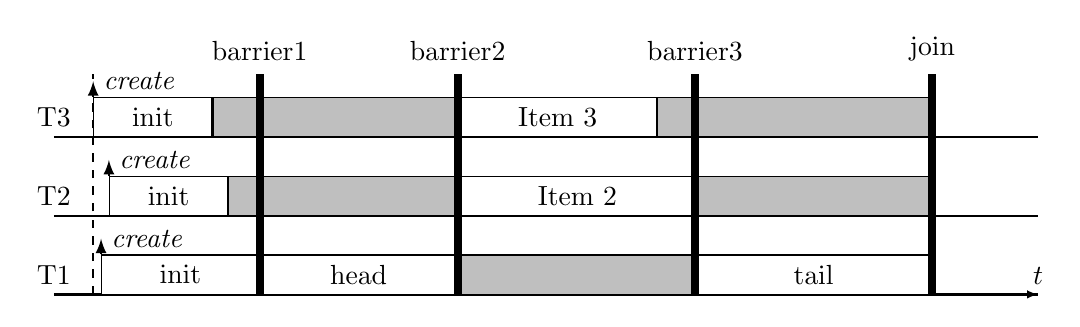
\begin{tikzpicture}[xscale=1,transform shape]

    \draw [-latex](-0.5,0) coordinate(dd)-- (0,0) coordinate (O1) -- (12,0)coordinate(ff) node[above]{$t$};
    \draw [dashed,thick] (O1) -- (0,0) coordinate(T1) -- (0,1) coordinate(T2) -- (0,2) coordinate(T3) -- ++(0,.8)coordinate(ff2);
    
    \foreach \nn in{T1,T2,T3}{
        \draw [thick] (dd|-\nn) node[above]{\nn}-- (\nn-|ff);
    }
    
    % \foreach \xx in{1,2,...,16}{
    % \draw[dashed] (\xx,0) -- (\xx,0|- ff2);
    % }
    
    % \foreach \xx in{0,4,8,...,16}{
    % \draw[dashed] (\xx,0.2) -- (\xx,-0.2) node[below]{\xx 0};
    % }
    
    \begin{scope}[shift={(T3)}]
        \node[ above right=0.25cm and 0cm of T3,right,draw, minimum width=1.5cm,minimum height=0.5cm,fill=white](T3start) {init};
        \node[ right=0cm of T3start,right,draw, minimum width=0.6cm,minimum height=0.5cm,fill=gray!50](T3w1) {};
        \node[ right=0cm of T3w1,right,draw, minimum width=2.5cm,minimum height=0.5cm,fill=gray!50](T3w2) {};
        \node[ right=0cm of T3w2,right,draw, minimum width=2.5cm,minimum height=0.5cm,fill=white](T3branch) {Item 3};
        \node[ right=0cm of T3branch,right,draw, minimum width=0.5cm,minimum height=0.5cm,fill=gray!50](T3w3) {};
        \node[ right=0cm of T3w3,right,draw, minimum width=3cm,minimum height=0.5cm,fill=gray!50](T3w4) {};
        \draw[-latex,thick] (T3start.north west) -- ++(0,0.2)node[right]{\emph{create}};
    \end{scope}
    
    \begin{scope}[shift={(T2)}]
        \node[ above right=0.25cm and 0.2cm of T2,right,draw, minimum width=1.5cm,minimum height=0.5cm,fill=white](T2start) {init};
        \node[ right=0cm of T2start,right,draw, minimum width=0.4cm,minimum height=0.5cm,fill=gray!50](T2w1) {};
        \node[ right=0cm of T2w1,right,draw, minimum width=2.5cm,minimum height=0.5cm,fill=gray!50](T2w2) {};
        \node[ right=0cm of T2w2,right,draw, minimum width=3cm,minimum height=0.5cm,fill=white](T2branch) {Item 2};
        \node[ right=0cm of T2branch,right,draw, minimum width=3cm,minimum height=0.5cm,fill=gray!50](T2w3) {};
        \draw[-latex,thick] (T2start.north west) -- ++(0,0.2)node[right]{\emph{create}};
    \end{scope}

    \begin{scope}[shift={(T1)}]
        \node[ above right=0.25cm and 0.1cm of T1,right,draw, minimum width=2.0cm,minimum height=0.5cm,fill=white](T1start) {init};
        \draw[-latex,thick] (T1start.north west) -- ++(0,0.2)node[right]{\emph{create}};
        \node[ right=0cm of T1start,right,draw, minimum width=2.5cm,minimum height=0.5cm,fill=white](T1neck) {head};
        \node[ right=0cm of T1neck,right,draw, minimum width=3cm,minimum height=0.5cm,fill=gray!50](T1w1) {};
        \node[ right=0cm of T1w1,right,draw, minimum width=3cm,minimum height=0.5cm,fill=white](T1head) {tail};
    \end{scope}
    
    \draw[line width=1mm] (T1start.south east) -- (T1start.south east |- ff2)node[above]{barrier1};
    \draw[line width=1mm] (T1neck.south east) -- (T1neck.south east |- ff2)node[above]{barrier2};
    \draw[line width=1mm] (T1w1.south east) -- (T1w1.south east |- ff2)node[above]{barrier3};
    \draw[line width=1mm] (T1head.south east) -- (T1head.south east |- ff2)node[above]{join};


    % Send variable arrow
    % \draw (T1neck.east) edge[-latex, bend left=45] (T2branch.west);
    % \draw (T1neck.east) edge[-latex, bend left=45] (T3branch.west);

\end{tikzpicture}
}
%      \caption{Global scheduling\label{fig-scheduling}}
\end{center}


The execution sequence 
starts with the 3 threads creation on the CPUs
and then reaches the first synchronization barrier.
Then Item1 thread calls the \emph{forward} method of layers of the head (until \emph{send\_var})
while Items 2 and 3 threads wait for the second synchronization barrier.
After,
the second synchronization barrier,
Items 2 and 3 threads  call \emph{forward} method of their layers
while Item1 thread waits for the third synchronization barrier.
After the third synchronization barrier,
Item 1 thread calls \emph{forward} method of layers of the tail.
At last, threads join and exit.




%####################################################################@
\subsection{Semantic preservation of the \petri net}
\label{sec-petriprese}
%We developed 3 instrumentation codes to validate the semantic preservation.
The first analysis
aims at verifying that all observed scheduling of layers on the \xavier
respects the \petri net semantics.
Because we use a static scheduler, all schedules should
behave as shown in section \ref{sec-petriprese}
which is included in the semantics of coloured \petri net
of figure \ref{fig:sync}.
% Thus we need to monitor the start and end of each branch/items. In each item, we need to monitor the execution of layers.
For that, we logged each start/end of branches and layers
and we stressed the robustness of the implementation by addind some temporal noises (sleep in the code).

All observed traces respected the schedule of section \ref{sec-petriprese}
with some timing variations.
When observing the implementation with no noise,
execution traces of Item 2 and 3 are interleaved on the \gpu.
When adding a wait of 1s at the beginning of Item 2
(just after barrier1), all layers of Item 3 were executed before those of Item 2. 

%% % Figure environment removed



\subsection{Semantics preservation of the function}
The second instrumentation mechanism aims at checking
that the functional semantics of the DNN is preserved.
We achieve this by re-implementing the \nnef specification in \pytorch. Then we define 100 random vectors that we run
both on the \pytorch implementation and on the C++ implementation on the \nvidia target. Finally, we compute the overall average error mean between both executions for the 100 runs. 

%We do not have access to the source code of convolution algorithms used by \cudnn
%or to convolution provided by \pytorch.
We were not able to find the exact convolution algorithm of \pytorch. We think that it exists a non documented heuristic that calls the best algorithm (considering execution time) depending of the convolution parameters and available hardware. 
According to the \cudnn documentation \cite{nvidiacudnn},
it is possible to select the convolution algorithm among a list, but details of the implementation are not given.
Thus, there may be a discrepancy between convolutions that we cannot fix.
The average error mean
is extremely small $1.10^{-7}$ for FLOAT32
using 3 \cudnn algorithms (namely gemm, Winograd and direct).
Nevertheless numeric precision results for this experiment are in an acceptable range that is very close to the available numeric precision of floating point representation
and
this also is observed by other frameworks \cite{SilvaCGP22}. 


\subsection{Measured Execution Time (MET)}
One objective of the DO-178C that we did not mention until now
is the capacity to estimate the Worst Case Execution Time (WCET). 
Due to the complexity of \nvidia target, a formal demonstration using static analysis %such as \otawa
may be difficult. But at least, a good property is a low variation of the measured execution time among several executions.
In our case, the generated code does not contain any IF-THEN-ELSE patterns
or dynamic loop conditions. Thus, the variability is only linked to the hardware behavior. 
We measured the MET of the complete DNN and of the first convolution of Item 1 over 10 runs.
We rely on the \emph{nsys} tool from \nvidia to get timing measurements.

\begin{center}
% \noindent\resizebox{.5\linewidth}{!}{
  \footnotesize
  \scriptsize

\begin{tabular}{|l|c|c|c|c|}
      \hline
       & \textbf{Mean(MET)} & \textbf{MIN(MET)} & \textbf{(MAX(MET))} & \textbf{STD(MET)} \\
      \hline
      \textbf{First Conv}  & 324 2976 ns  & 322 688 ns & 326 656 ns  & 1.45 ns \\
      \textbf{DNN}  &  24 257 $\mu$s &  16 285 $\mu$s &  53 950 $\mu$s & 13 526 $\mu$s\\
      \hline
  \end{tabular}
\end{center}

%Results show  mean, min, max and std measurements of the execution time for the first convolution and the whole pipeline.
The MET of the first convolution is very stable with a very low jitter.
The MET distribution of the DNN is large
and to understand why, we need to investigate the low level behaviour.
\nvidia\ \gpus are  black-boxes processors on which we cannot guarantee worst-case execution time \cite{AmertA21,carle-erts22}.
%This perfectly illustrate issues that we may encounter when using complex hardware whereas software algorithms are without any branches.
%For a compliant DO178C this behavior need to be understood and an effort shall be put in limiting this global jitter.

% Whereas the error is extremely 
% https://docs.nvidia.com/deeplearning/cudnn/api/index.html#cudnnConvolutionFwdAlgo_t



% Rajouter des expes sur le profiling avec nvprob

Most academic vocabulary lists have been developed in the context of English for Academic Purposes (EAP). On the whole, two categories of lists exist. One list type aims to identify academic words commonly used in EAP across disciplines, which students could be made aware of. The studies aiming to provide cross-disciplinary academic word lists usually use large corpora containing expert academic writing from various disciplines. The widely used lists of this type are the Academic Word List (AWL) \cite{coxhead2000new} and the Academic Vocabulary List (AVL) \cite{gardner2014new}. The second type of list seeks to identify discipline or field-specific words worth teaching. Various specialised lists have been developed for fields such as veterinary medicine \cite{ohashi2020esp} or nursing \cite{yang2015nursing}.

While there is a growing interest in building cross-disciplinary academic word lists for languages other than English, these academic word lists remain few. See, for example studies conducted for French \cite{cobb2004there}, Persian \cite{rezvanifirst}, Portuguese \cite{baptista2010p}, Swedish \cite{carlund2012academic}, and Norwegian \cite{johannessen2016constructing}. An explanation for this scarcity might be that academic language data sets are rare and often not freely available due to copyright. This can be especially true for low-resource languages, such as Romanian. Access to a representative corpus is crucial, as the validity and reliability of an academic word list highly depend on the quality of the data set. 

Apart from the limited availability of academic writing corpora, an additional challenge may be that there is no standard procedure for extracting academic word lists. Scholars are still exploring and testing various methodologies. For example, some studies build on the methods used for the AWL or the AVL \cite{johannessen2016constructing,rezvanifirst}. One study uses the translated version of the AVL in Portuguese as a starting point for its investigation \cite{baptista2010p}. Another study proposes a new word list extraction method different from previous ones \cite{carlund2012academic}.  

In the case of Romanian, no previous studies have compiled specialised or general academic word lists. Although in the last 10-15 years, several research institutions and projects have been involved in developing corpus resources in Romanian, relatively few have focused exclusively on general academic writing. Some of the most significant corpora recently compiled, such as ROMBAC (Romanian Balanced Annotated Corpus, see \citet{ion2012rombac}), with more than 30 million words, CoRoLa (Corpus of Contemporary Romanian Language, see \citet{mititelu2014corola}), or The Balanced Romanian Corpus (BRC, see \citet{midrigan2020resources}) cover only few disciplines or subsets: 5 sections for ROMBAC (journalism, literature, medical texts, legal texts, biographies), uneven and unfiltered distribution of resources in CoRoLa (the collection of academic writing texts is based on agreements with publishing houses and journals, without filtering of the content on quality criteria) and BRC (literary text samples, research articles, news, spoken data). The ROMBAC corpus (excluding the medical subcorpus) was already used to develop the Romanian Word List (RWL, see \citet{szabo2015introducing}), targeted at Romanian L2 learners (e.g. from the Hungarian minority in Romania). The list is a general list of words, not focused on academic language. As far as discipline-specific corpora are concerned, smaller corpora such as SiMoNERo (medical corpus, \citet{mitrofan2019monero}), BioRo \cite{mitrofan2018bioro}, PARSEME-Ro (news articles), LegalNERo (legal, \citet{paiș2021named}), MARCELL (legal, multilingual, see \citet{varadi2020marcell}), CURLICAT (multilingual, containing several domains: Economics, Education, Health, Sciences, etc., see \citet{varadi2022introducing}) have been compiled. However, apart from compiling the datasets and conducting a series of descriptive studies, no special attention is given to the lexical level. 

In this context, the EXPRES corpus (Corpus of Expert Writing in Romanian and English) is the first corpus of discipline-specific academic writing in the Romanian context (academic writing in Romanian L1 and academic writing in English L2 produced by Romanians) \cite{bucur2022expres,chitez2022write}. Covering four disciplines – Linguistics, Economics, Political Sciences, Information Technology –, the Romanian subset contains 200 open-access research articles from each domain, published in the past 5-10 years in peer-reviewed journals (see \citet{chitez2022expres}). The rigorous selection criteria \cite{rogobete2021challenges} contribute to the representativeness of the corpus, making it a suitable candidate for testing a possible Romanian Word List and narrowing it down to an Academic Word List. Furthermore, the EXPRES corpus is the first Romanian expert academic corpus available on an open-access query platform. Unlike other Romanian corpora, which offer limited access to third parties and poor resources for downloading search results or statistics, the EXPRES corpus support platform has been implemented as a cross-platform distributed web application  \cite{chitez2022expres}.

\section{Conclusion and Future Work}
In this work, I design corruption-robust algorithms for the Lipschitz contextual search problem. I present the \emph{agnostic checking} technique and demonstrate its effectiveness in designing corruption-robust algorithms. There are several open problems for future research. First, in the algorithm I propose for pricing loss, the schedule for agnostic checks is fixed upfront. Can the learner design an adaptive checking schedule for the pricing loss? Second, this work assumes the learner has knowledge of the Lipschitz constant $L$. Can the learner design efficient no-regret algorithms without knowledge of $L$? 

{\footnotesize
\subsection*{\textbf{Acknowledgments}}
This work has benefited from the AI Interdisciplinary Institute ANITI,
funded by the  “Investing for the Future – PIA3” program
Grant agreement ANR-19-P3IA-0004 and
from  the PHYLOG 2 project funded by the French government through the France Relance program, based on the funding from and by the European Union through the NextGenerationEU program.}



\bibliographystyle{alpha}
\bibliography{bib}


\end{document}
